The development of this project is structured into distinct phases, following an iterative methodology to ensure the integration of complex vision language models with robotic simulation. However, the planning also allows to go back to previous steps of the project development to refine or change points completed in the past, in order to iteratively enhance the performance and quality of the end result. Finally, a Gantt graph (\ref{fig:gantt_diagram}) will be available to illustrate the progression of project divided tasks.

\section{Task division}
The tasks will be divided by project area, and each will contain a brief description and amount of time spent on it. The final results will be available at table \ref{tab:phases_hours}.

\subsection*{Phase 1: Theoretical research}
Focus on studying the theoretical foundations of the project and the best tool options to tackle the challenge.
\begin{itemize}
	\item \textbf{Research of VLMs}: investigate what VLMs are and how they work, plus options to integrate them in a practical way.
	
	\item \textbf{RL framework research}: check for the best options to integrate vision language models into robotic environments.
	
	\item \textbf{State-of-the-art review}: comparative analysis of existing models and papers.
\end{itemize}

\subsection*{Phase 2: Experimentation}
Start experimenting with basic VLM implementation and the principles of IsaacSim.
\begin{itemize}
	\item \textbf{Foundational VLM tasks}: first visual question answering, image captioning tests.
	
	\item \textbf{IsaacSim tutorials}: follow up of the official documentation tutorials and YouTube videos to get familiar with the framework and its functionalities.
	
	\item \textbf{Local Model Deployment}: setting up the local environment and running the first inferences with the first VLMs outside of the simulation.
	
	\item \textbf{Basic Scene Scripting}: testing Python snippets to manipulate simple objects within the scenario and experiment with the VLM captioning asset inside Isaac Sim.
\end{itemize}

\subsection*{Phase 3: Architecture design}
Designing the communication bridge between the high-level reasoning and the low-level simulation.
\begin{itemize}
	\item \textbf{BentoML server architecture}: design of a local BentoML server to handle asynchronous requests, experimenting with different functionalities and features.
	
	\item \textbf{Coordinate transformation logic}: mathematical definition of the function used to transform the predicted VLM coordinates into real scenario points.
	
	\item \textbf{Workflow pipeline design}: iterative development of different workflow pipelines. 
\end{itemize}

\subsection*{Phase 4: Solution development}
Technical implementation of the simulation environment and the agent logic.
\begin{itemize}
	\item \textbf{Scenarios development}: design of progressively more complex scenarios, starting from the very basics up to multi-agent environments. 
	
	\item \textbf{RL policy training}: training of different policy trainings, tweaking different hyperparameters, rewards and approaches.
	
	\item \textbf{Prompt Engineering Refinement}: developing specific system prompts for the VLM to improve detection accuracy in industrial contexts. 
	
	\item \textbf{Robot Control Integration}: linking the unprojected coordinates to the Franka Emika and Jetbot motion controllers, creating custom classes and functions for each case.
\end{itemize}

\subsection*{Phase 5: Results evaluation \& refinement}
Analysis of the system's performance and iterative enhancement.
\begin{itemize}
	\item \textbf{Performance evaluation}: measuring the success rate of the VLM-guided tasks and calculating the error margin in detection tasks.
	
	\item \textbf{Implementation of improvement techniques}: design of new alternative techniques to improve the performance of VLM detection.
	
	\item \textbf{Comparative analysis}: comparing the performance of different model versions or prompt strategies.
\end{itemize}

\subsection*{Phase 6: Documentation}
Summary of the research, development, and results into the final report.

\subsection{Planification table}

The following table quantifies the dedication required for each of the major blocks of the project. 


\begin{table}[H]
	\centering
	\small
	\begin{tabularx}{10cm}{X r}
		\toprule
		\textbf{Phase} & \textbf{Estimated Hours} \\
		\midrule
		Theoretical research & 15h \\
		\midrule
		Experimentation & 45h \\
		\midrule
		Solution development & 120h \\
		\midrule
		Results evaluation \& refinement & 90h \\
		\midrule
		Documentation & 60h \\
		\midrule
		\textbf{Total Estimated Workload} & \textbf{330h} \\
		\bottomrule
	\end{tabularx}
	\caption{Table indicating the time spent in each major phase of the project.}
	\label{tab:phases_hours}
\end{table}

\clearpage
\begin{sidewaysfigure}
	\centering
	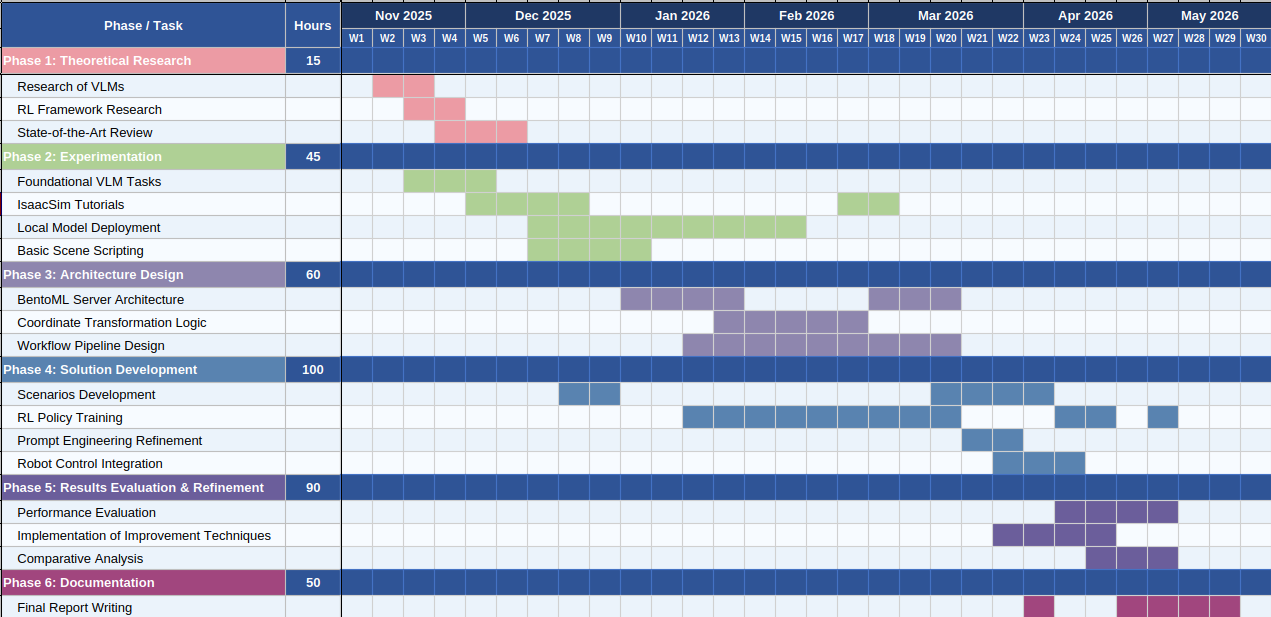
\includegraphics[width=.9\textwidth]{imgs/gantt.png}
	\caption{Project development timeline using a Gantt chart.}
	\label{fig:gantt_diagram}
\end{sidewaysfigure}